\documentclass[10pt,letter]{article}
	% basic article document class
	% use percent signs to make comments to yourself -- they will not show up.

\usepackage{amsmath}
\usepackage{amssymb}
	% packages that allow mathematical formatting

\usepackage{graphicx}
	% package that allows you to include graphics

\usepackage{setspace}
	% package that allows you to change spacing

\onehalfspacing
	% text become 1.5 spaced

\usepackage{fullpage}
	% package that specifies normal margins
	
\usepackage[version=3]{mhchem} % Package for chemical equation typesetting
\usepackage{graphicx} % Required for the inclusion of images
\usepackage{natbib} % Required to change bibliography style to APA
\usepackage{amsmath} % Required for some math elements 
\usepackage{booktabs}
\usepackage{floatrow}
	

\begin{document}
	% line of code telling latex that your document is beginning


\title{CS 156 Problem Set 7}

\author{Christopher Zhen}

\date{Nov 14, 2016}
	% Note: when you omit this command, the current dateis automatically included
 
\maketitle 
	% tells latex to follow your header (e.g., title, author) commands.
	
\section*{Problem 1}

\textbf{(D)} - According to our code, when $k = 6$, we have a classification error of 0 in the validation set which is the best of the choices.

\section*{Problem 2}

\textbf{(E)} - According to our code, when $k = 7$, we have a classification error of $0.076$ which is the lowest of the answer choices. This shows that our validation set was not very good at predicting the output data.

%\begin{figure}[H]
%\begin{center}
%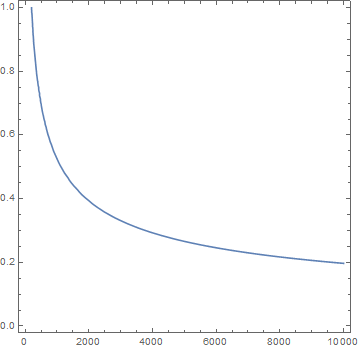
\includegraphics[width=0.5\textwidth]{2d.png}
%\caption{Table courtesy of the textbook %textit{Learning from Data}.}
%\label{2d}
%\end{center}
%\end{figure}

\section*{Problem 3} 

\textbf{(D)} - Once again, according to our code when $k = 6$ we have the lowest classification error in the validation set of $0.0833$.

\section*{Problem 4}

\textbf{(D)} - This time, when $k = 6$ we also get the lowest classification error on the output set, though the error this time is $0.192$ which is significantly higher than before which means our training set was not an accurate approximation of the output set.

\section*{Problem 5}

\textbf{(B)} - Our errors of $0.076$ and $0.192$ are closest to answer choice B.

\section*{Problem 6}

\textbf{(D)} - It makes sense for the expected value of e to be lower than 0.5 since there's a min function. According to the code, e should be around 1/3 which makes sense and is closest to answer choice D.

\section*{Problem 7}

\textbf{(C)} - See attached sheet.

\section*{Problem 8}

\textbf{(C)} - Using our code (implementing the sklearn package) we get that around 56\% of the time SVC is more accurate than PLA which is closest to answer choice C.

\section*{Problem 9}

\textbf{(D)} - The code returned 62.1\% which is closest to answer choice D.

\section*{Problem 10}

\textbf{(B)} - The code returned a value of 2.97 which is closest to answer choice B.

\end{document}
	% line of code telling latex that your document is ending. If you leave this out, you'll get an error
